We present here the expected work plan for this master's thesis. A description of the activities can be found in Section~\ref{sec:Methodology}
\begin{figure}[h]
	\centering
	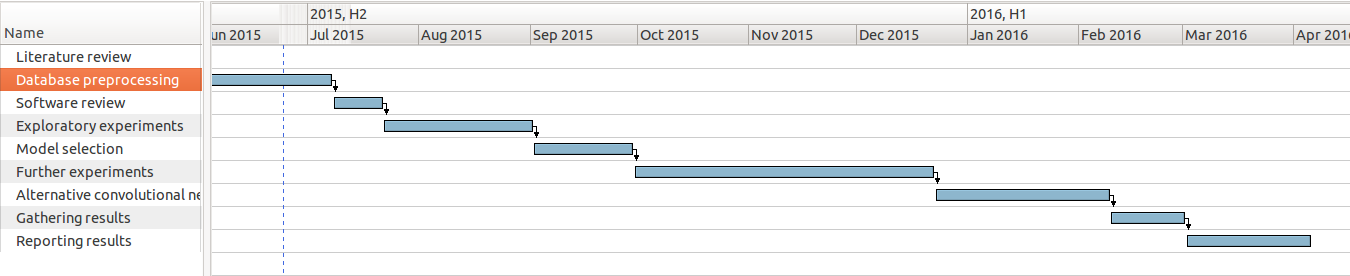
\includegraphics[width = \textwidth]{plots/workplan.png}
	\caption[Thesis Work Plan]{Thesis work plan.}
	\label{fig:workplan}
\end{figure}

\begin{comment}
Una vez establecida la {\it Metodología} es importante establecer las
actividades con sus tiempos respectivos en lo que se llama el {\it Plan de
Trabajo}. Ello nos da una idea clara de la extensión en tiempo del trabajo
propuesto. Además de ser necesario, lo cual es normalmente cierto en
propuestas de proyecto industrial, es importante establecer el PLAN FINANCIERO
el cual desglosa los recursos necesarios para el desarrollo del proyecto y sus
costos.

{\bf Un ejemplo de Plan de Trabajo}

La figura \ref{ttphd} presenta el cronograma de las actividades que llevarán a
cabo los objetivos de esta tesis. 

\begin{figure}[th]
	\centerline{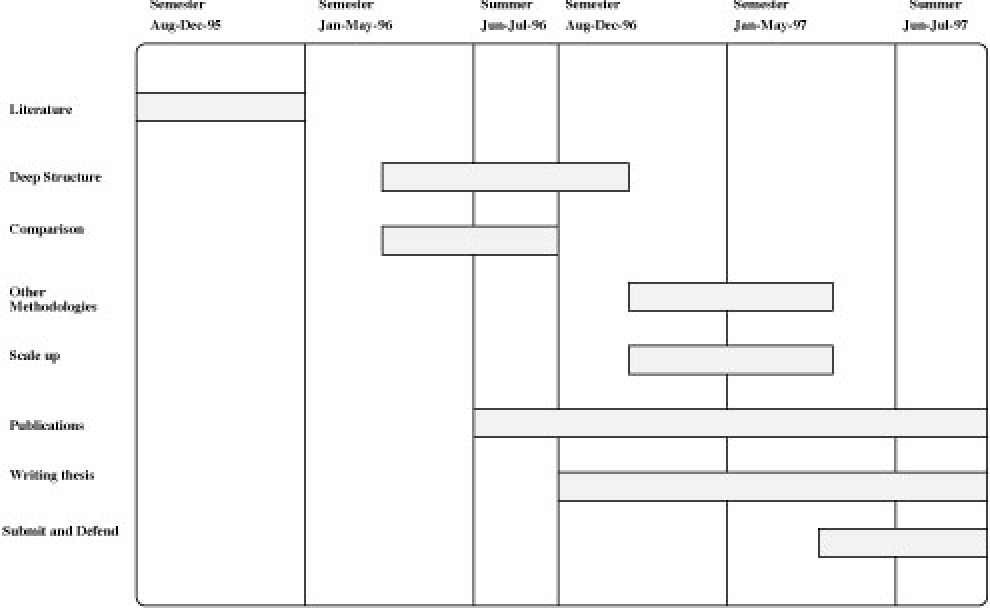
\includegraphics[width=4in,height=3in]{plots/ttphd.pdf}}
	\caption{Cronograma de Actividades para desarrollar la Tesis}
	\label{ttphd}
\end{figure}
\end{comment}
